\section{Task 2 --- Generating a Certificate Request for Your Web Server}
%
\begin{lstlisting}[language=bash,caption=A command generating CSR for the server]
openssl req -newkey rsa:2048 -sha256 \
    -keyout server.key -out server.csr \
    -subj "/CN=www.student22.com/O=Student22 Inc./C=US" \
    -passout pass:dees \
    -addext "subjectAltName = DNS:www.student22.com,\
                            DNS:www.student22cuong.com,\
                            DNS:www.student22mahibul.com"
\end{lstlisting}

\begin{figure}
    \centering
    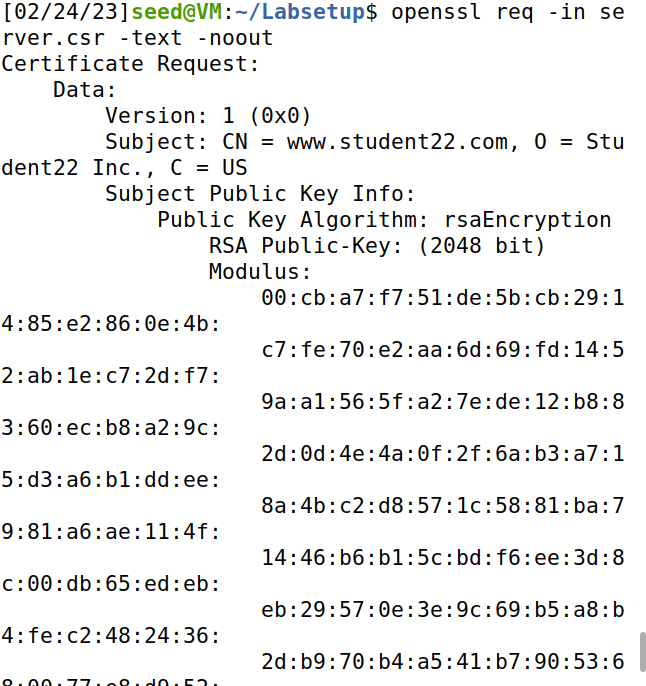
\includegraphics[height=\textheight,width=\textwidth,keepaspectratio]
    {figures/server_csr.png}
    \caption{Certificate Signing Request for the server
    {\fontfamily{qcr}\selectfont www.student22.com}.}
    \label{fig:server_csr}
\end{figure}

Two alternative names, {\fontfamily{qcr}\selectfont www.student22cuong.com} and
{\fontfamily{qcr}\selectfont www.student22mahibul.com}, are included
in the {\fontfamily{qcr}\selectfont openssl ca} command.
\autoref{fig:server_csr} shows partly the Certificate Signing Request
(CSR) for the server {\fontfamily{qcr}\selectfont www.student22.com}.